\chapter{Fundamente Teoretice și Stadiul Actual}
\label{chap:fundamente_teoretice}

\section{Propagarea Undelor Radio în Spații Închise}
Propagarea undelor electromagnetice în interiorul clădirilor (\textit{indoor multipath propagation}) este guvernată de o combinație complexă de fenomene fizice: reflexie pe pereți și obiecte metalice, refracție prin materiale dielectrice, difracție pe margini ascuțite și dispersie datorată suprafețelor neregulate.

Într-un mediu indoor tipic, semnalul radio emis de o antenă transmițătoare ajunge la antena receptoare nu doar pe calea directă de vizibilitate directă (LoS -- \textit{Line-of-Sight}), ci pe o multitudine de căi indirecte (NLoS -- \textit{Non-Line-of-Sight}). Fiecare cale de propagare $i$ este caracterizată printr-o atenuare specifică $a_i(t)$, o întârziere de propagare $\tau_i(t)$ și un defazaj indus $\theta_i(t)$. Semnalul receptat în domeniul timpului reprezintă convoluția dintre semnalul emis $s(t)$ și răspunsul la impuls al canalului $h(t)$:
\begin{equation}
    y(t) = s(t) * h(t) = \sum_{i=1}^{N_p} a_i(t) s(t - \tau_i(t)) e^{-j \theta_i(t)} + n(t)
    \label{eq:channel_impulse_response}
\end{equation}
unde $N_p$ reprezintă numărul de căi de propagare, iar $n(t)$ este zgomotul alb gaussian aditiv (AWGN).

Când un corp uman se interpune pe una sau mai multe căi de propagare, atenuarea și lungimea fazică a acelor căi suferă variații substanțiale din cauza permitivității dielectrice ridicate a țesutului biologic ($\epsilon_r \approx 50$ la frecvența de 2.4 GHz, datorită conținutului ridicat de apă). Astfel, corpul uman acționează ca un reflector și atenuator dinamic de radiofrecvență.

\section{De la RSSI la CSI: Granularitatea Informației Radio}
\subsection{Limitările Indicatorului RSSI}
Istoric, primele sisteme de detecție și localizare radio s-au bazat pe indicatorul de putere a semnalului recepționat (RSSI -- \textit{Received Signal Strength Indicator}). Deși RSSI este accesibil pe orice placă de rețea comercială fără modificări firmware, utilitatea sa pentru detecția mișcărilor fine și a căderilor este sever limitată:
\begin{enumerate}
    \item \textbf{Metrică scalară agregată:} RSSI măsoară puterea totală recepționată, cumulată pe întreaga bandă a canalului (de exemplu 20 MHz), integrând toate căile multipath într-o singură valoare scalară în dBm.
    \item \textbf{Vulnerabilitate extremă la fading destructiv:} O variație infimă a poziției unei căi de reflexie poate cauza interferență destructivă, prăbușind RSSI-ul cu până la 15--20 dB chiar și în absența oricărei mișcări a utilizatorului.
    \item \textbf{Rată mică de raportare:} De regulă, RSSI este actualizat doar o dată per pachet sau la nivel de beacon (10 Hz), insuficient pentru captarea dinamicii rapide a unei căderi ($<1\text{ s}$).
\end{enumerate}

\subsection{Channel State Information (CSI) în Modulația OFDM}
Standardul IEEE 802.11n/ac utilizează modulația cu diviziune ortogonală a frecvenței (OFDM -- \textit{Orthogonal Frequency Division Multiplexing}). Canalul de 20 MHz este divizat în 64 de subpurtătoare ortogonale și paralele. Dintre acestea, 52 de subpurtătoare transportă date active și piloți de sincronizare (indexate în gama $[-26..-1]$ și $[+1..+26]$, subpurtătoarea 0 reprezentând purtătoarea continuă nulă DC).

Pentru fiecare subpurtătoare $k \in \{1, \dots, 52\}$, egalizatorul receptorului Wi-Fi estimează funcția de transfer complexă a canalului $H(f_k)$:
\begin{equation}
    Y(f_k) = H(f_k) \cdot X(f_k) + N(f_k)
\end{equation}
unde $X(f_k)$ este simbolul emis cunoscut, $Y(f_k)$ simbolul recepționat, iar $N(f_k)$ componenta de zgomot.

Valoarea CSI $H(f_k)$ este un număr complex ce comprimă două dimensiuni fundamentale:
\begin{equation}
    H(f_k) = |H(f_k)| e^{j \angle H(f_k)}
\end{equation}
\begin{itemize}
    \item $|H(f_k)| = \sqrt{I_k^2 + Q_k^2}$ reprezintă \textbf{amplitudinea CSI}, reflectând atenuarea indusă de mediul fizic pe frecvența $f_k$;
    \item $\angle H(f_k) = \arctan\left(\frac{Q_k}{I_k}\right)$ reprezintă \textbf{faza CSI}, reflectând defazajul geometric total parcurs de frontul de undă.
\end{itemize}

Deoarece fiecare subpurtătoare are o frecvență centrală distinctă $f_k = f_c + k \cdot \Delta f$ (cu $\Delta f = 312.5\text{ kHz}$ în 802.11n), lungimile de undă asociate diferă subtil. Acest fenomen permite matricei CSI să funcționeze ca un spectrometru radio de înaltă rezoluție, rezolvând efectul multipath și izolând mișcările corpului uman cu precizie milimetrică \cite{wang2015understanding}.

\section{Modelul Zonelor Fresnel și Cartografierea 2D}
Zona Fresnel reprezintă regiunea tridimensională concentrică de formă elipsoidală din jurul liniei drepte care unește emițătorul ($Tx$) și receptorul ($Rx$), în interiorul căreia undele reflectate ajung la receptor cu o diferență de fază determinată.

\begin{figure}[H]
    \centering
    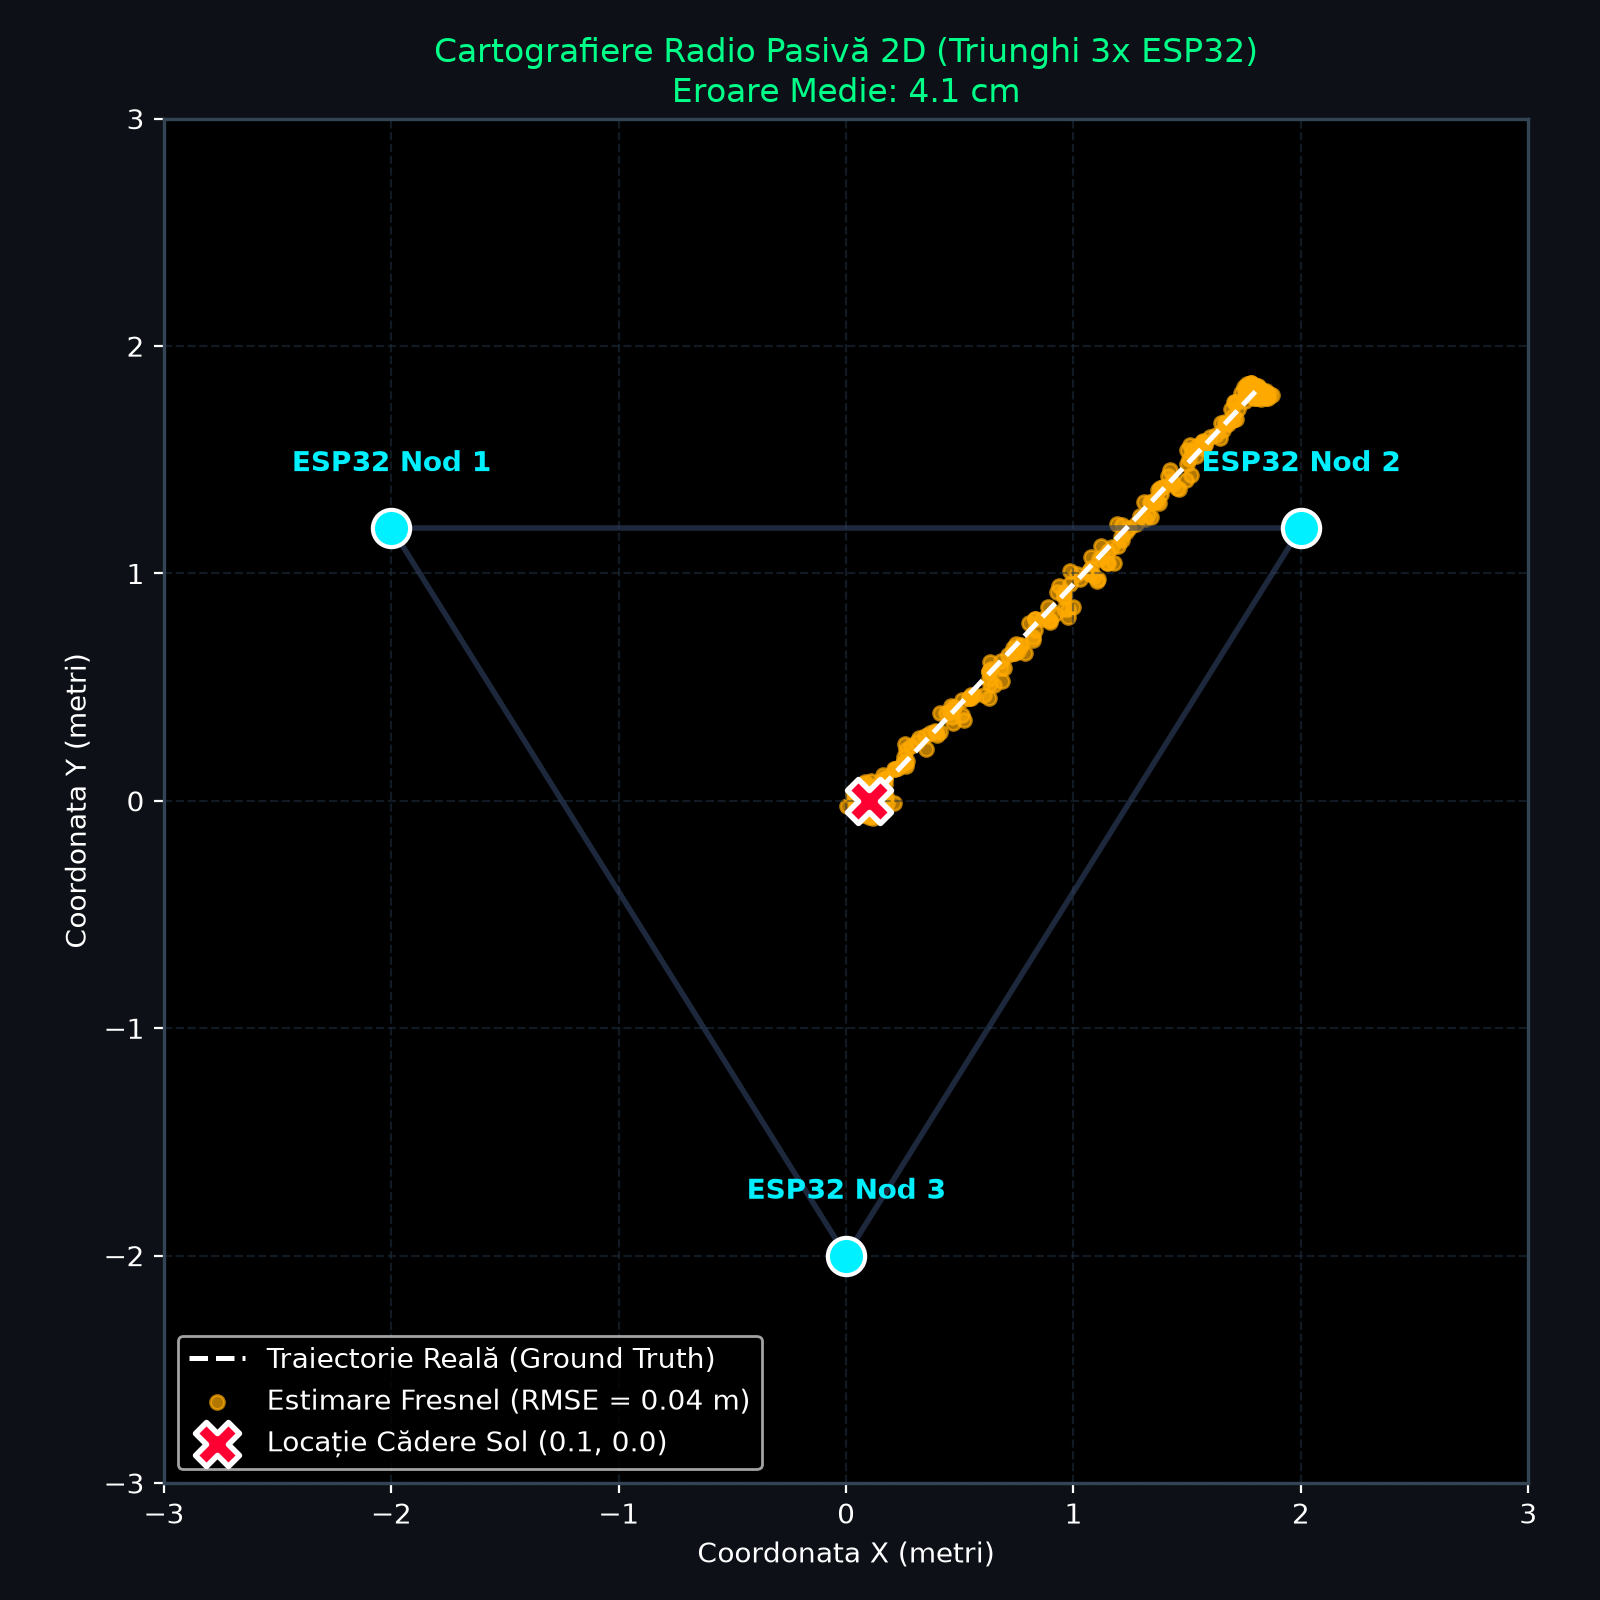
\includegraphics[width=0.75\textwidth]{figures/3_trajectory_cartography.png}
    \caption{Cartografierea traiectoriei 2D și intersecția elipselor confocale formate de topologia triunghiulară a nodurilor radio.}
    \label{fig:trajectory_cartography}
\end{figure}

Pentru a $n$-a zonă Fresnel, lungimea traiectoriei reflectate $d_1 + d_2$ depășește distanța directă $d$ cu un multiplu de jumătate de lungime de undă $\lambda$:
\begin{equation}
    d_1 + d_2 - d = n \frac{\lambda}{2}, \quad n \in \{1, 2, 3, \dots\}
    \label{eq:fresnel_definition}
\end{equation}
Raza maximă a celei de-a $n$-a zone Fresnel la o distanță $d_1$ de $Tx$ și $d_2$ de $Rx$ este dată de formula:
\begin{equation}
    r_n = \sqrt{\frac{n \lambda d_1 d_2}{d_1 + d_2}}
\end{equation}

Pentru banda de 2.4 GHz, lungimea de undă este:
\begin{equation}
    \lambda = \frac{c}{f} = \frac{3 \times 10^8\text{ m/s}}{2.4 \times 10^9\text{ Hz}} = 0.125\text{ m} = 12.5\text{ cm}
\end{equation}

Dacă o persoană traversează granița dintre zonele Fresnel (adică o distanță de $\lambda / 2 \approx 6.25\text{ cm}$), semnalul reflectat alternează între interferență constructivă ($n$ par) și interferență destructivă ($n$ impar). Această alternanță produce o sinusoidă clară în anvelopa amplitudinii CSI. Prin amplasarea a trei noduri în triunghi, se obțin trei perechi de focare eliptice distincte ($L_{12}, L_{23}, L_{31}$). Intersecția suprafețelor modulate energetic identifică univoc poziția țintei în plan 2D \cite{wu2017device}.

\section{Efectul Micro-Doppler în Dinamica Căderii}
Când un obiect sau un membru corporal se deplasează cu viteza liniară $v$ într-un câmp radiofrecvență, frecvența undei recepționate suferă o deplasare Doppler $f_D$:
\begin{equation}
    f_D(t) = \frac{v(t)}{\lambda} (\cos \alpha + \cos \beta)
\end{equation}
unde $\alpha$ și $\beta$ sunt unghiurile dintre vectorul viteză și direcțiile către emițător, respectiv receptor.

În timpul activităților casnice uzuale:
\begin{itemize}
    \item \textbf{Mersul normal:} Viteza centrului de masă este cuprinsă între $0.8\text{ m/s}$ și $1.4\text{ m/s}$. Aceasta corespunde unei frecvențe Doppler de bază de aproximativ $10 - 18\text{ Hz}$, cu modulații periodice produse de mișcarea membrelor inferioare.
    \item \textbf{Căderea necontrolată:} Reprezintă o prăbușire verticală accelerată gravitațional ($g \approx 9.81\text{ m/s}^2$). În faza de impact, capul și toracele ating viteze de $2.5 - 4.5\text{ m/s}$, generând o explozie spectrală Doppler scurtă (sub $400\text{ ms}$) cu frecvențe de vârf ce depășesc $35 - 50\text{ Hz}$.
\end{itemize}

Această disparitate cinematică pronunțată constituie baza fizică a separării căderilor reale de acțiunile benigne de așezare pe scaun sau mers accelerat.

\section{Analiza Comparativă a Literaturii de Specialitate}
Tabelul \ref{tab:literature_comparison} sintetizează principalele abordări din literatura academică de profil în raport cu soluția propusă în prezenta teză.

\begin{table}[H]
\centering
\small
\begin{tabular}{@{}lllll@{}}
\toprule
\textbf{Sistem / Lucrare} & \textbf{Hardware Utilizat} & \textbf{Metrică Radio} & \textbf{Metodologie} & \textbf{Limitare Cheie} \\ \midrule
Wi-Vi (2013) \cite{adib2013see} & USRP SDR (scump) & Fază / RSSI & Anulare LoS analogică & Echipamente greoaie, cost ridicat \\
PhaseBeat (2017) \cite{wang2017phasebeat} & Intel 5300 NIC & Fază diferențială CSI & FFT Respirație/Puls & Necesită cablu ceas comun între antene \\
FarSense (2018) \cite{zeng2018farsense} & Intel 5300 NIC & CSI-Ratio & Model elipsoidal & Doar monitorizare respirație statică \\
WiVib (2020) \cite{zhang2020wivib} & Atheros AR9580 & CSI Amplitudine & Micro-Doppler & Diagnostic utilaje, nu detecție căderi \\
ESPARGOS (2023) \cite{schon2023espargos} & Matrice ESP32 & AoA / CSI & Antenă phased-array & Complexitate RF hardware ridicată \\
\textbf{Sistemul Propus} & \textbf{3x ESP32 + Ubertooth} & \textbf{CSI 52 subpurt.} & \textbf{FSM Multi-Link + STFT} & \textbf{Cost sub \$30, timp real 60 FPS} \\ \bottomrule
\end{tabular}
\caption{Comparație sintetică între soluțiile existente în literatură și sistemul realizat.}
\label{tab:literature_comparison}
\end{table}
